\section{Implementation}
\label{sec:impl}

We describe four key aspects of our implementation:
\if 0
how the uncertainty-aware model is efficiently constructed and maintained (\S\ref{sec:statemachine}), 
mechanisms to bound temporary uncertainty (\S\ref{sec:bound}),
an optimization on our storage data structure to accelerate verification (\S\ref{sec:trie}),
\wxznew{and an extension of the model to support bandwidth checking (\S\ref{sec:bandwidth}).}
\fi
\kevin{
1) how to efficiently construct and maintain the uncertainty-aware model,
2) how to bound temporary uncertainty,
3) how to accelerate verification with storage data structure optimization,
and 4) how to support bandwidth checking.
}

%\subsection{Uncertainty State Machine}
%\subsection{Representing Network Uncertainty}
%\label{sec:statemachine}

\paragraphb{Representing Network Uncertainty.}
In our uncertainty graph, we need to keep track of the state of each link.  
%At first glance, we can do this by keeping a simple {\em state machine} for each link, which has two states: certain, and uncertain.  However, two states are not sufficient, as there are some complexities which arise in practice.  For example, there may be dependencies across updates -- the question of whether to mark a link as certain can depend on updates that follow.  
\kevin{However, simply keeping two states, certain and uncertain, are not sufficient (e.g., whether to mark a link as certain can depend on subsequent updates).}
%\mattc{To address this, we need to construct a correct and more general state machine to represent link status.}
% matt: post sigcomm, I don't get how general this is or if it's more than just for duplicate updates.
%-- suppose two duplicate add rules (the same rule being added to the network twice, to refresh state), followed by a delete.
%If the delete was not present, as soon as the first update was confirmed, the second update could be assumed to be co
%
%In addition, if two rule 
%
%need to keep track of when a rule is certain and when it is uncertain
%two states not enough
%- delete and add can't be reordered
%- suppose we send several updates to add rules
%suppose there are N which add the same rul on diff devices
%we get N-1 confirmations from that rule
%-- send rule repeatedly to avoid expiry - or app just does it
%--- you send two duplicate adds to the network, followed by a delete
%if you didn't have the delete, as soon as you got an ack for the first update, you could assume the second update arrived too
%if you do have the delete, you need to treat the link as uncertain because the seconde add could still be in flight
%
%
%
%we need a state machine
%if you build that state machine in a naive way you have large nubmer of states - problem because implementation becomes more complex and error prone, and memory requiremsnet become larger, 
%to deal with this we come up with a clever way to store states

%Based on functionalities of the Trie data structure, 
%we implement our uncertainty aware network modeling technique.
%In the uncertainty-aware graph model,
%as described in \S~\ref{sec:design}, 
%links in the graph model are labeled as either certain or uncertain.
Therefore, \name keeps track of the state of each rule, and associate
them each with a status of uncertainty as well as two counters.  The status of
uncertainty could be one in the set \{\emph{uncertain, certain, pre-certain, unknown}\}. 
The counter, \emph{add\_cnt}, records the number of
insertions of the rule, and the counter, \emph{del\_cnt} records the number of
deletions. 
%If one rule is modified to another rule, then the first rule's \emph{add\_cnt} decreases by one, and the second rule increases its \emph{del\_cnt}.

Figure~\ref{fig:statemachine} shows the state machine of our uncertainty-aware
model. The \emph{certain} and \emph{uncertain} states are consistent
with the notion during modeling phase. The \emph{pre-certain} and
\emph{unknown} \matt{require some additional explanation, which we will clarify
through an example. } Suppose that rule (update) $R$ is issued by the
controller. Before the controller receives an acknowledgment of $R$, the
status of $R$ in our \cut{trie} storage data structure (discussed later in
\S\ref{sec:trie}) is \emph{uncertain} and its \emph{add\_cnt} counter increases
from zero to one.  Once $R$ is confirmed, %later before any other action on $R$ happens, 
$R$'s status is changed to \emph{certain}, and the \emph{add\_cnt}
counter is \matt{reset} to zero.  If another insertion of $R$ is issued
before the first $R$ is confirmed, then the status of $R$ remains
\emph{uncertain}, and the \emph{add\_cnt} counter is increased to two. Assume
one confirmation is received now. We are certain that $R$ exists in the
network, but there is an in-flight control message to add $R$ again, which may
conflict with a later deletion.  Such case is represented by the status
\emph{pre-certain}. Note that if a rule is \emph{pre-certain} for adding action
(\emph{Add\_pre\_certain}), it is certainly included in the model. Similarly,
if a rule is in the state \emph{Del\_pre\_certain}, then the rule is not
modeled.  The status, \emph{unknown}, describes the case that the same rule is
first added and then deleted (or the other way round), but the controller has
not yet received a confirmation of the first command\cut{, and not yet issued the
second command}. Hence, the order of applying the two \matt{in-flight} commands
is unknown, even after both commands are acknowledged.
\wxzc{One reviewer had a comment about this paragraph.}

\begin{figure}[!ht]
  \centering
  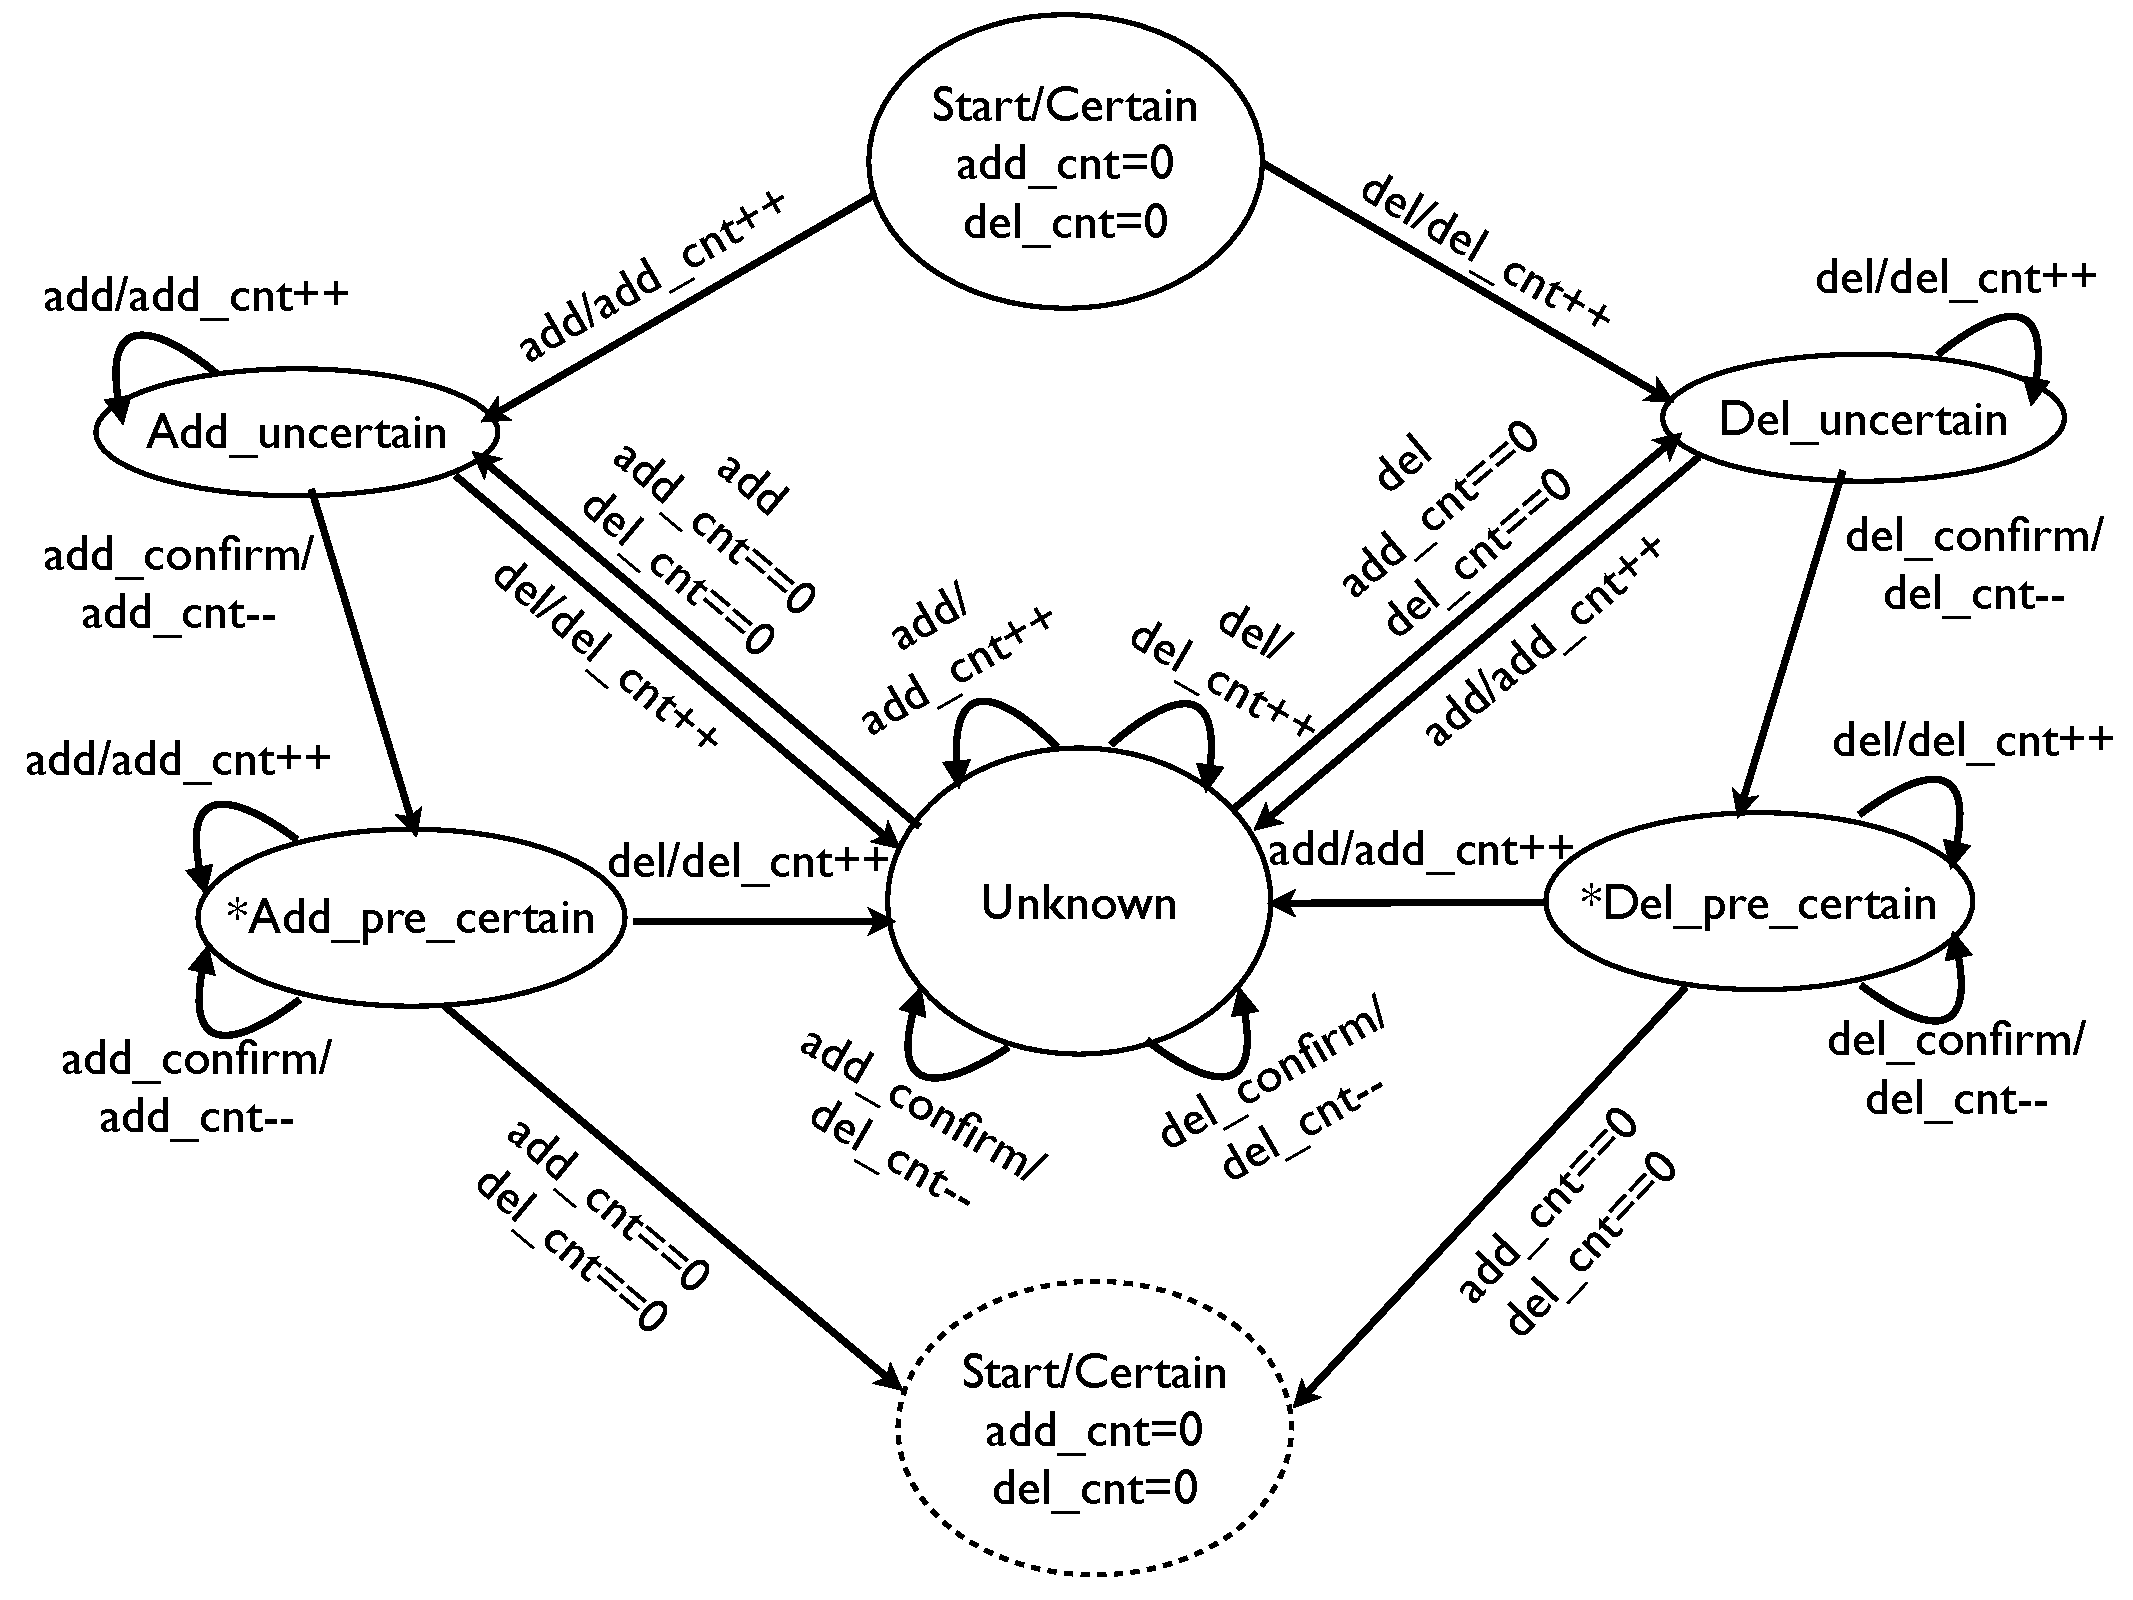
\includegraphics[width=\columnwidth]{figs/statemachine}
  \vspace{-0.3in}
  \caption{\em Uncertainty state machine}
  \label{fig:statemachine}
\end{figure}

%\subsection{Bounding Network Uncertainty}
%\label{sec:bound}
%move to implementation
%\subsection{VeriFlow}
%\label{sec:veriflow}
%As the foundation of our work, we first briefly introduce VeriFlow, a real-time network-wide verifier.
%Sitting between the controller and the network, VeriFlow intercept every update issued by the controller before it hits the network and verify its effect in real-time through the following three steps.

%First, VeriFlow slices the entire packet space into a set of Equivalence Classes (ECs) of packets
%using all existing forwarding rules and the new update.
%Each of the ECs is a set of packets that experience the same forwarding actions throughout the network.
%Because each update typically affects a very small number of ECs, 
%to limit searching space,
%VeriFlow only focuses on ECs that might be influenced by the new update. 
%Second, VeriFlow builds a forwarding graphs for each of the affected ECs respectively, 
%representing forwarding behaviors of packets belonging to those ECes.
%Last, VeriFlow traverses each of these graphs,
%to verify network-wide invariants.

%No acknowledgments. Switches do not acknowledge when FlowMod messages are processed, except when errors occur. 

%\wxzc{from spec}
%If the controller has requested to be noticed when fow entries time out or are deleted from tables, the datapath does this with the OFPT_FLOW_REMOVED message.
%Flow entries are removed from ow tables in two ways, either at the request of the controller or via the
%switch ow expiry mechanism.The controller may actively remove ow entries from ow tables by sending
%delete fow table modification messages (OFPFC_DELETE or OFPFC_DELETE_STRICT)
% Each flow removed message contains a complete description of the ow entry,
% the reason for removal (expiry or delete), the ow entry duration at the time of removal, and the ow
% statistics at the time of removal.
% ow table entry is identied by its match elds and priority: the match elds and priority taken
% together identify a unique ow entry in the ow table. The ow entry that wildcards all elds (all elds
% omitted) and has priority equal to 0 is called the table-miss ow entry.
% ˆ Flow Entry: an element in a flow table used to match and process packets. It contains a set of
% match fields for matching packets, a priority for matching precedence, a set of counters to track
% packets, and a set of instructions to apply.
% ˆ Match Field: a field against which a packet is matched, including packet headers, the ingress
% port, and the metadata value. A match field may be wildcarded (match any value) and in some
% cases bitmasked.
%

\paragraphb{Bounding Network Uncertainty.} To bound the amount of time that the controller is uncertain about network states, 
a mechanism to acquire \matt{{\em confirmations} (an indication that the rule has been applied in the network)} is required.  
%However, 
Although existing SDN protocols such as OpenFlow
do not support general application layer acknowledgments~\cite{openflow-spec},
\cut{
Let us take the flow entry change as an example. Switches typically only acknowledge rule removals, but not for rule insertions or modifications~\cite{openflow-spec}.
However, }
there are other options,
% to implement the acknowledgment mechanism by, 
for example,
(1) making use of the barrier and barrier reply messages of OpenFlow protocol,
(2) leveraging an appropriately-chosen timeout
%The controller can explicitly request acknowledgements by sending a barrier request after issuing a command to a network device. The device will respond with a barrier reply after it processes this command and all other messages before it.
or (3) having the controller actively query the data plane.
\cut{
In addition, if future SDN protocols explicitly allow switches
to acknowledge control messages, we can leverage this in our design.
These options present a tradeoff in terms of control overhead, delay, and so on.
%(3) extending SDN protocols to allow switches explicitly acknowledging control messages,
%or (3) making the controller query the data plane actively.

%Among these options, the third one is most expensive in terms of control overhead and delay. The second option requires no modification on the protocol, and the additional delay is as small as the first option. However, the second option doubles the number of extra control messages that are needed by the first option. 

\matt{To gain some understanding of the tradeoffs involved,}
} 
We implemented two versions of the confirmation mechanism:
%First, we built 
an application-level acknowledgment \cut{mechanism} by modifying the Stanford OpenFlow switch reference implementation, 
(tested with a Mininet-based emulation), and
%. The other version is 
a mechanism leveraging the barrier and barrier reply messages
%implemented 
on our physical SDN testbed.%~\cite{ocean}, 
%\mattc{is there a good reason why you did two different versions? Maybe to gain experience with the tradeoffs involved?}

%\subsection{Efficiently Storing State}
%\label{sec:trie}
%1. rule data structure
%originally, strings are used to present "match". It was slow. Now we use 64 bit unsigned integers to do the same operations, and allows bit operation tricks.
%Storage is saved. IP, 32bit int only needs 4 bytes, but instead string needs more than 10bytes.
%
%The way to store rule is improved. Trie itself has match info, so we don't need keep an extra copy of match at leaves, only need to store the part of rules other than match at leaves.
%In this way we save 16byte*14(fields) overhead.
%In addition, a trie leave stores a hash table, indexed by device ip to distinguish rules on different devices. This is far more efficient than storing raw rules on leaves.
%
%2. insertion, search, deletion all use sentinel and bit operation to speed up.
%Using sentinels saves the cost of checking branch conditions.
%Plus, reduce the number of copy operations.

%3. traverse trie only once for each update
%Vanilla VF traverses the trie first to computed affected EC ranges, then does the second traversal to collect rules, which is both memory expensive and slow.
%Instead we use callback functions to implement one time trie traversal algorithm:
%...
%
%4. optimizing wildcard and
%
%%Field         Description
%%OXM_OF_IN_PORT        Ingress port. This may be a physical or switch-defined logical port.
%%OXM_OF_ETH_DST        Ethernet destination address. Can use arbitrary bitmask
%%OXM_OF_ETH_SRC        Ethernet source address. Can use arbitrary bitmask
%%OXM_OF_ETH_TYPE       Ethernet type of the OpenFlow packet payload, after VLAN tags.
%%OXM_OF_IP_PROTO       IPv4 or IPv6 protocol number
%%OXM_OF_IPV4_SRC       IPv4 source address. Can use subnet mask or arbitrary bitmask
%%OXM_OF_IPV4_DST       IPv4 destination address. Can use subnet mask or arbitrary bitmask
%%OXM_OF_IPV6_SRC       IPv6 source address. Can use subnet mask or arbitrary bitmask
%%OXM_OF_IPV6_DST       IPv6 destination address. Can use subnet mask or arbitrary bitmask
%%OXM_OF_TCP_SRC        TCP source port
%%OXM_OF_TCP_DST        TCP destination port
%%OXM_OF_UDP_SRC        UDP source port
%%OXM_OF_UDP_DST        UDP destination port
%
%different head fields correspond to different type of wildcard: full wildcard, ip wildcard, and bitwise whildcard. Most fields use the first.
%
%For case 1, maintain a wildcard table and a binary search tree. Insertion, deletion and search operations only require an additional condition.
%For rules with wildcard, traverse all leaves plus the wildcard table.
%
%For case 2, because except the non-wildcarded prefix, the following bits are wildcarded, it is a generalized form of case 1.
%At the leaves of the current level trie, a wildcard table is stored.
%Note here, the height of the trie is not fixed, and can be less than the number of bits of the corresponding packet header, unlike VF.%depends on the wild card bits of rules
%
%Case 3 is the most troublesome. During traversals, if some bit is non-wildcard, for example, 0, then traversing both 0 branch and wildcard branch. 
%Otherwise first traverse 0+wildcard branches, then 1+wildcard.

% 
% \mattc{
% We need to maintain state efficiently
% There's several pieces of state that veriflow matains
% - list them out - 5 of them
% 4 of those are easy to do.
% but the 5th one is the bottleneck - which efficiently traversing the state to do xxx
% 
% ther eare existin galgorithms to efficinetly comptue reachabaility on graphs
% for example: veriflow and hsa
% unforutnatley, we have an added challenge of doing a larger search
% which increases the computation time challenges
% to address this we came up wwith a more efficeint data structure
% 
% key insight: veriflow does a two pass algorithm
% but you can comptue3 the same thign you compute with two passes with one pass
% first pass is to compute EC sets
% second pass is to find rules influencing that ec
% we utilize the trie data structure to do both at once
% }

\paragraphb{Efficiently Storing State.} There are several pieces of state that \name maintains, including network-wide data plane rules, uncertainty state of each rule, and buffered updates. The key bottlenecks arise during the computationally-challenging procedure of storing and processing data plane rules.
%the data plane rules: both during the process of determining how many
%  different uncertain forwarding views in current network, and the process of
%  traversing uncertain graphs built on these views.}

%\mattc{can you add any quick results on memory usage? even just run top and report the number you see there?}
%\wxzc{540MB vs 9GB}
%\mattc{ok that's great -- and you already mentioned it in the text, I forgot}

%\mattc{it also seems like this section conflicts with your story about "black box" -- how can yo uclaim you're treating verification as a black box with all these modifications you make to it? -- can deal with this after sigcomm} REVISIT

%\name requires the ability to store and process information about network states.
%Given the need to store multiple different representations of the network, this state
%could be larger than just storing a single snapshot.
%To mitigate this, we construct an efficient data structure and traversal process for our core algorithms.

The way that \name stores and retrieves data plane rules is motivated by Veriflow~\cite{VeriFlow}. 
The essential idea is to build a multiple-layer trie, with each layer sub-trie representing a packet header field. 
\if 0
Each level of a sub-trie corresponds to a bit of that \cut{packet header} field.
%and can be one of three possible values: $0$, $1$, or wildcard.
An upper layer sub-trie contains pointers on leaves to sub-tries in the next layer. 
Dataplane rules are stored at the leaves of bottom sub-tries.
A path from the root to a leaf of a bottom sub-trie determines a packet set, and one or more such sets can be merged together to form an \emph{equivalence class} (EC) of packets, \matt{i.e.,}
%More formally, an \emph{equivalence class} (EC) is 
a set of packets experiencing the same behaviors \wxznew{throughout the network}\cut{at any network device}.
Upon arrival of an update, its effect on the network state is checked, by limiting searching to ECs whose behavior may be affected by this update, and building a graph model for each affected EC.
\fi
However, given the need to store \cut{multiple}different representations of the network state, the storage and processing overhead of \name could be larger than just maintaining a single snapshot as done in Veriflow. \kevin{Moreover, we need to handle rules that perform packet transformation, such as Network Address Translation.}
%Moreover, there are rules that perform packet transformation, such as Network Address Translation, i.e., those rules transform packets from one EC to another EC. To accurately model network behaviors, we need to able to handle such rules, which are left out in our motivating work, Veriflow.
\cut{To meet this end,} In \name, we have designed a scalable data structure and an efficient algorithm to operate on it.
%to to model network state.%for our network modelling technique. 

%- wildcards make traversal complicated
%- because need to traverse multiple branches
%- three wildcard types - some fields have any bits wc, some are longest prefix match
%-- define what each is
%- bitmask - may have to traverse mult branches
%- full wildcard - whole filed is dc or none is - optimization helps perfomance
%- subnet mask - optimization
%-- those cases come up a lot in practice

\paragraphe{Customized Trie Data Structure.}
%To scale the data structure,
%besides the general type of trie, we design two types of customized trie structure. 
\matt{\cut{
To achieve scale, we design a customized trie structure.
We start with a standard trie. However,} 
One complication is dealing with {\em wildcards} -- rules agnostic to matching on certain bits
or fields. Wildcards complicate the traversal process, as multiple branches may need to be traversed, and the manner
in which they are traversed can depend on the semantics of the rule (e.g., standard wildcards vs. longest-prefix match).
To address this, we construct an algorithm that handles general bitmasking, then extend it with optimizations
to more efficiently handle two common-case wildcard patterns: full wildcards (the entire field is wildcarded) and subnet mask (all bits
less than a certain significance are wildcarded).  }
%and corresponding traversal algorithms,
%\mattc{is there missing text here? the following sentence is incomplete and I don't get the connection with what preceeds it}
%for three wildcard types of packet header field supported in OpenFlow protocol~\cite{openflow-spec}:
%\mattc{I suddenly get lost here. You started talking about tries. What do tries have to do with wildcards? Are you saying something like you use a trie, but %there's some additional complexity in handling wildcards? What complexity is that? Need to say it explicitly.}
%bitmask, subnet mask and full wildcard, respectively.
%For a field that supports bitmask, i.e., wildcard bits can be set with no restriction, the general trie data structure is used, and each trie node has three children %branches, $0$, $1$ and wildcard. 
%Subnet wildcard field is a general wildcard type, used mostly for IP related match fields. 
%In subnet wildcard field, the wildcard bits can only appear after non-wildcard fields, and all follow up bits must be wildcard. In the customized trie structure for %this type of field,
%each node also has 
%\mattc{missing text here?}
To deal with wildcarding for bitmasks, each node in our trie has three child branches, one for each of \{0,1,don't care\}. For subnetting, the wildcard branch has no children but points direct to a next layer sub-trie or a rule set.
Thus, unlike other types of trie, 
the depth of subnet wildcard tries is not fixed as the number of bits in this field, 
but instead equals to the longest prefix among all the rules it stores.
Accordingly, traversal cost is reduced compared with general tries.
As for the full wildcard field, values can only be non-wildcarded or full wildcarded.
The specialized trie structure for this type of field is a plain binary tree plus a wildcard table.
%Compared to tools that don't consider network uncertainty, \name faces 
%But in \name, things are more challenging: because of the confirmation
%mechanism, rules tend to stay longer in the Trie, and in turn create more ECs
%than in VeriFlow. Moreover, due to the uncertainty of data plane rules, there
%might be more than one possible path for the matched packets to get forwarded.
%These paths should all be traversed to check if problems might raise, which in
%the worst case need to traverse every node in the uncertain graph. These
%challenges, if not properly handled, will prevent \name operating in real time.

%To address these problems, we build upon similar methods used in Veriflow, but
%with much more optimizations. 
\paragraphe{One-pass Traversal Algorithm.}
When a new update arrives, we need to determine the set of affected \cut{Equivalence
Classes }ECs, as well as the rules \cut{affected by} \wxznew{affecting} those ECs.
Veriflow~\cite{VeriFlow} performs a similar task via a two-pass algorithm,
first traversing the trie to compute a set of ECs, and then for each of the
discovered ECs, traversing the trie again to extract related rules.  In \name,
we optimize this process by maintaining some additional accounting information,
which lets us accomplish our similar objective in a single pass.  
Our algorithm starts from the top layer subtrie, and combinations
of its branches that match the first field of the update to be checked are
selected.  The traversal continues on the matched combinations, and would be
further confined by the following fields of the update.  A matched combination
of branches in the last level is an EC, and it already points to the rule set
for that EC.  Using callback functions and depth first searching, we
implemented in place checking, and finish the modeling work with only one
traversal.  This algorithm eliminates both the unnecessary extra pass over the
trie and also the need to allocate memory for intermediate results.  In
addition, this approach results in a smaller number of ECs---each wildcard
branch itself forms a matched combination.

\wxznew{
After getting the rule set for each EC, \name traverses the 
graph model consisting of the collected rules, to check network invariants.
One special case is dealing with packet transformation rules. 
When such a rule is encountered during graph traversal phase, a new pass over the trie
for the transformed EC is triggered. 
Note that the graph is constructed while traversing rules, so only rules encountered 
before transformation are kept, and the remaining rule set is discarded.
More importantly, in this case, multiple trie traversals are possible, but only when 
necessary, i.e., when a transformation rule is possibly forwarding packets for the original EC.
} 
%For an incoming update, determining the affected ECs and rules influencing those ECs simultaneously is difficult, because rules that may take effect on one EC could spread widely in the Trie, not only on the branches defining the EC. As a result, VeriFlow~\cite{VeriFlow} chooses to first traverses the Trie to compute a set of ECs, and for each of these ranges/ECs, it traverse the Trie oncemore to extract related rules.

% However, by fully leveraging the trie structure, we can avoid
% %both redundantly splitting ECs and 
% multiple Trie traversals.
% To do this, our algorithm starts from the top layer sub-Trie, and
% combinations of its branches that match 
% %can be partitioned by matching 
% the first field of the update to be checked are selected. 
% The traversal continues on the matched combinations, and would be further confined by the following fields of the update. 
% A matched combination of branches in the last level is an EC, and it already points to the rule set for that EC. 
% Using callback functions and depth first searching, we implemented in place checking, 
% and finish the modeling work with only one traversal.
% This algorithm eliminates both the unnecessary extra pass over the trie and also the need to allocate memory for intermediate results. 
% 
% A byproduct of the one-pass traversal algorithm is a reduced number of ECs. 
% The way VeriFlow computes EC sets is likely to split larger ECs into smaller pieces.
% For example, consider a three-bit-wide field (eight possible values). 
% In the data plane, five rules that match $000, 010, 100, [110-111]$, 
% and full wildcard `*' in this field respectively, are present.
% To check the impact of a new rule with full wildcarded `*' match, seven disjoint ranges ($000, 001, 010, 011, 100, 101, [110-111]$) are considered as ECs.
% But note that the ranges $001, 011, 101$ can be combined to one EC, as all matching packets would be handled by full wildcard rules.
% The extra number of ECs could slow down the performance significantly,
% as the runtime cost is basically linear to the number of ECs~\cite{VeriFlow}. 
% more memory for holding intermediate results. 
% Fortunately, using our algorithm, the wildcard branch itself forms a matched combination, resulting only five ECs.

%Veriflow uses a two phase algorithm ---the first
%determines what ECs exist in the network. The second pass finds a set of rules
%that influence corresponding EC. 
%To optimize this process for our domain, we developed a one-pass traversal algorithm, which finds matching rules in
%parallel with discovering ECs~\ref{sec:traverse}. 
%This effort eliminates both
%the unnecessary extra pass and the need to allocate memory for temporary
%results. 
%Moreover, we designed partition algorithms based on sub-Trie's
%characteristics~\ref{sec:wildcard}, and can produce fewer ECs than VeriFlow.
%Lastly, in \name we no longer build the whole forwarding graph, but only lazily
%retrieving needed rules, and this can remove useless actions.

These efforts together with a highly optimized implementation 
allow \name to run almost 100X faster compared to Veriflow
%despite having all the challenges we listed.
with 15X less memory overhead% (540MB vs. 9GB).
(\S\ref{sec:microbenchmark}). 
One of our ongoing works is exploring the parallel implementation of the data structure.

\wxznew{
%\subsection{Checking Bandwidth Properties}
%\label{sec:bandwidth}

\paragraphb{Checking Bandwidth Properties.}
Thanks to \name's graph-based model, it is straightforward to incorporate bandwidth information to the model.
To keep tract of bandwidth usage, besides forwarding graphs, \name also maintains a network-wide physical topology graph.
Whenever a set of rules are issued to set up paths for flows with bandwidth requirement, 
\name reserves bandwidth on all possible paths taken by those flows on the physical graph model.
As rules are confirmed to be removed, \name releases bandwidth occupied by flows that these rules used to forward.
\wxzc{assumption: we can get bandwidth info for flows at gcc level.}
Results shown previously (\S\ref{sec:synthesis}) on the integration of \name and SWAN proves the feasibility of this implementation.
}

%%%But 
%%%, and an MEC is an EC that cannot be divided further on rule insertions.
%%To speed up verification processing, like VeriFlow, we developed
%%
%%
%%we confine it to ECs, whose
%%actions may be influenced by a new update.  That is, upon the arrival of an
%%update, only rules overlapping with its affected ECs are retrieved from the
%%Trie, to build up the network model to verify.  However, several facts prevent
%%VeriFlow from reaching the microsecond-per-update level processing time:
%%
%%\begin{itemize}
%%  \item Two-pass traversal algorithm. Veriflow computes 
%%    the set of EC(s) to check, and then extracts the rules affecting
%%    each EC. This method does not take full advantage of the special Trie structure. 
%%    Compared with the one-pass algorithm that \name uses, this not only increases
%%    run time, but also needs more memory to hold temporary traversal results.
%%  \item Strictly Sequential Execution.
%%  %\item Some implementation details, such like too many object copies in C++, and
%%  %  unnecessary branch conditions.
%%\end{itemize}
%%
%%In \name, we implement a similar Trie data structure for storing and
%%retrieving data plane rules, but with a one-pass traversal algorithm,\mattc{what is a "pass"? what do you mean by one-pass? you never said veriflow does multiple passes} 
%and highly optimized implementation. 
%\if 0
%\mattc{if you're short on space, shorten the remainder of this section:}
%
%Originally:
%To speed up verification processing, like VeriFlow,
%we confine it to ECs, whose actions may be influenced by a new update.
%That is, upon the arrival of an update, only rules overlapping with its affected ECs 
%are retrieved from the Trie, to build up the network model to verify.
%However, several facts prevent VeriFlow from reaching the micro-second-per-update-level processing time:
%
%\begin{itemize}
%  \item Two-pass traversal algorithm. Veriflow computes numeric ranges to
%    determine which EC(s) to check, and then extracts the rules affecting
%    each EC. This method does not take full advantage of the special Trie structure. 
%    Compared with the one pass algorithm that \name uses, this not only increases
%    run time, but also needs more memory to hold temporary traversal results.
%  \item Strictly Sequential Execution.
%  %\item Some implementation details, such like too many object copies in C++, and
%  %  unnecessary branch conditions.
%\end{itemize}
%
%In \name, we implement a similar Trie data structure for storing and
%retrieving data plane rules, but with a one-pass traversal algorithm, 
%and highly optimized implementation.  This enables \name to run
%almost 100x faster than VeriFlow release code(\S~\ref{sec:microbenchmark}) despite
%having network uncertainty modelled and checked. 
%Moreover, our implementation uses 15X less memory than VeriFlow during checking(540MB vs 9GB). 
%One of our ongoing works is exploring the parallel implementation of the data structure. 
%
%\paragraph{One Pass Traversal Algorithm}
%
%%For an incoming update, determining the affected ECs and rules influencing
%%those ECs simultaneously is difficult.  Because of wildcard bits, rules that
%%may take effect on one EC could spread widely in the Trie, not only on the
%%branches defining the EC. 
%%To solve these problems, VeriFlow chooses to first traverses
%%the Trie to find out each ECs, and then based on these EC to retrieve all
%%the rules stored on leaves level.
%
%For an incoming update, determining the affected ECs and rules influencing
%those ECs can be done at the same time. Two pass algorithm like what is in
%VeriFlow will waste not only one extra pass traversing on the Tire, but also
%more memory for holding intermediate results. What is the worst is that the
%range based algorithm may create potentially more ECs than \name. For example,
%Suppose in the data plane only exist five rules that match ranges $000, 010,
%100, [110-111]$, and full wildcard `*' in this field. Then when a new update
%coming with '*' set in this field, too, an optimal partition will be(``$000,
%010, 100, [110-111]$''). But range based method can not achieve this accuracy.
%Instead in VeriFlow, it will only create more ECs to check against:``$000,
%001, 010, 011, 100, 101, [110-111]$''.

%
%Originally:
%For an incoming update, determining the affected ECs and rules influencing those ECs simultaneously is difficult. 
%Rules that may take effect on one EC could spread widely in the Trie, not only on the branches
%defining the EC.
%As a result,  VeriFlow~\cite{VeriFlow} first traverses the Trie 
%to compute a set of disjoint rule match ranges as ECs. 
%However, the range sets computed in this way actually splitting larger ECs into smaller pieces.
%For example, a three-bit-wide field has eight possible values. 
%Suppose in the data plane only exist five rules that match ranges $000, 010, 100, [110-111]$, 
%and full wildcard `*' in this field.
%To check the impact of a new rule with full wildcard `*' match, seven disjoint ranges ($000, 001, 010, 011, 100, 101, [110-111]$) are considered as ECs.
%But note here the ranges $001, 012, 101$ can be combined to one EC, as matching packets would be handled by full wildcard rules.
%The extra number of ECs could slow down the performance significantly,
%as the runtime cost is basically linear to the number of ECs~\cite{VeriFlow}. 
%Next, for each of these ranges/ECs, it pays another pass to extract related rules.
%
%We can avoid both redundantly splitting ECs and multiple Trie traversals by fully leveraging the Trie structure.
%To obtain affected ECs and related rules, we argue that it is enough to traverse the Trie just once.
%Starting from the first layer of sub-Trie,
%it could be partitioned by matching the first field of the rule to verify. 
%The matched partitions could be further divided and confined by the following fields. 
%A partition in the last level is an EC, and it already points to the rule set for that EC. 
%Using callback functions and depth first searching, we implemented in place checking, 
%and finish the modeling work with only one traversal.
%
%%\wxzc{Add some thing about why we need to "add" the check rule?}
%
%
%\mattc{why did you do that? needs more context}
%\fi
%and we will discuss the details as follows.
%following section. Pseudo code is listed in
%appendix (FIXME A) for interested readers, and due to space limit, we
%will not prove these algorithms.


%Because of wildcard bits, rules that
%may take effect on one EC could spread widely in the Trie, not only on the
%branches defining the EC. To solve these problems, VeriFlow~\cite{VeriFlow} chooses to first traverses
%the Trie to find out each ECs, and then based on these EC to retrieve all
%the rules storead on leaves level.
%
%However, the range sets computed in this way splits larger ECs into smaller pieces.
%For example, a three-bit-wide field has eight possible values. 
%Suppose in the data plane only exist five rules that match ranges $000, 010, 100, [110-111]$, 
%and full wildcard `*' in this field.
%To check the impact of a new rule with full wildcard `*' match, seven disjoint
%ranges ($000, 001, 010, 011, 100, 101, [110-111]$) are considered as ECs.  But
%note here the ranges $001, 012, 101$ can be combined to one EC, as matching
%packets would be handled by full wildcard rules, and it also adds the number of
%total ECs.
%The extra number of ECs could slow down the performance significantly,
%as the runtime cost is basically linear to the number of ECs~\cite{VeriFlow}. 
%Next, for each of these ranges/ECs, it pays another pass to extract related rules.

%We can avoid both redundantly splitting ECs and multiple Trie traversals by
%fully leveraging the Trie structure.  To obtain affected ECs and related rules,
%it is enough to traverse the Trie just once.  Starting from the first layer of
%sub-Trie, it could be partitioned by matching the first field of the rule to
%verify.  The matched partitions could be further divided and confined by the
%following fields.  A partition in the last level is an EC, and it already
%points to the rule set for that EC. Using callback functions and depth first
%searching, we implemented in place checking, and finish the modeling work with
%only one traversal.

%One thing to note is here a partition may contain multiple sub-tries or rule sets. 
%They could logically be combined to a larger trie or a rule set. When we describing
%the partition algorithm, we will assume we have only one trie to traverse.

%\paragraph{Full Wildcard}
%The full wildcard header field can only contain non-wildcard values or full wildcard
%value `*'. The specialized trie structure for this type of field is a plain binary
%tree plus a wildcard table.
%, with the tree leaves and the wildcard branch pointing to next layer tries or rule sets. 
%When a non-wildcard rule joins, the corresponding leaf and the wildcard branch
%together form the only matched partition at this layer. 
%If the incoming rule matches `*' in this field, 
%each combination of any individual leaf and the wildcard branch is checked one by one.

%For non-wildcard value V, suppose the corresponding leaf of V is L, then the only
%XX for V is composed by sub-Trie(or rule set) pointed by L and the wildcard
%branch. For '*', a XX is similar, but there would be multiple XX, equal to the
%number of leaves. This can be accomplished in one pass DFS.

%A special case is the wildcard branch itself forms a matched partition. 
%This happens when there is no leaf that corresponds to some non-wildcard match value, 
%and there exists rules in the wildcard branch. 
%Take the above three-bit-wide field example again.
%Once a wildcard rule is checked, the matched partitions using our searching algorithm 
%is optimal: $000, 010, 100, [110-111]$ and $[001, 011, 101]$.

%\paragraph{Subnet Wildcard}
%Subnet wildcard field is a general wildcard type, used mostly for IP related match fields. 
%The wildcard bits can only appear after non-wildcard fields, and all follow up bits must be wildcard.
%For this type of field, its trie contains a wildcard branch on every node, . 
%So an 8-bit field with value/mask 0xc0/0xf0 will be stored in path
%1-1-0-0's wildcard branch.
%In subnet wildcard type trie, each node contains at most two children and a wildcard branch.
%Leaves of the trie and wildcard branches on all nodes point to next layer tries or rule sets.
%The location to store a rule is determined by its non-wildcard bits in this field. 
%For example, when a rule that matches IP field `255.0.0.0/8' is to be inserted, 
%it will follow the path 1-1-1-1-1-1-1-1 to the wildcard branch there.
%Note that unlike other fields, the depth of subnet wildcard tries is not fixed as the number of bits in this field, 
%but instead equals to the longest prefix of all the rules. 
%Accordingly, traversal cost is reduced compared with uncustomized tries.

%During traversals, each matched partition is constructed in following
%way. First we traverse from the root to the node representing the last non-wildcared bit, 
%and collect the wildcard branches along the path as one set.
%Then the union of this set and the wildcard branches on
%the path from the current node to each leaf makes one partition, respectively.
%In this way, we are able to find all matched partitions. Moreover, 
%the number of the found partitions are optimal, in the sense that any two partitions
%cannot be combined.
%Using above principles, XX belong to this layer will also be partitioned optimal.
%Partition IP wildcard fields will be a little more troublesome than full
%wildcard fields. Assume the incoming rule is R, and X.next means the next
%layer Trie pointed by a Trie node X. Then there are several steps to find out
%each XX:

%\begin{itemize}
%\item Locate the Trie node T where R is stored. During this process, collect
%all X.next for X on the path of root->T. Record this set as WS.
%\item Perform DFS down from node T. At each node N, add N.next to WS on
%entering, and remove N.next on leave. Also,
%\begin{itemize}
%\item if N is a leaf, WS forms a XX, and mark N as checked
%\item if N has only one children, and N.next is NULL, then mark N as unchecked.
%\item if N has only one children, and N.next is not NULL, then current
%WS forms a XX, and mark N as checked.
%\item if N has two children, then recursively visit both children in DFS order.
%If one child is unchecked, and N.next is not null, then WS is a XX; else,
%mark N as unchecked.
%\end{itemize}
%\end{itemize}
%
%Using above principles, XX belong to this layer will also be partitioned optimal.


%\paragraph{Bitmask Wildcard}
%For general wildcard fields, 
%Wildcard bits can be set with no restriction. 
%In this case, we maintain three children per trie node, $0$, $1$ and wildcard.
%As traversing from the root to leaves, we check all possible unions of branches
%that overlap with the rule using depth-first search algorithms, and output a set of sub-trie or rule set partitions.
%Assume the field length is L, and field value is val. Then the algorithm to partition is:
%\begin{itemize}
%\item maintain a stack Q with (\{root\},L) as init value.
%\item pop out (V,l) from Q while Q is not empty
%\item if l is 0, then all the next layer Trie in V forms a XX
%\item else if l is a non wildcard bit, then push (V', l-1) on Q. V' is composed by
%to N.children[val[l]] and N.children['*'] for all nodes N of V.
%\item else if l is a wildcard bit, then push (V', l-1), (V'',l-1) on Q. Here
%V' is same as above, and V'' contains N.children[1 - val[l]] and N.children['*']
%for all nodes N of V.
%\end{itemize}
%
%The current partitioning algorithm is not optimal for such Tries, i.e., the partitions are not a minimal set.
%One of our ongoing works is to investigate techniques to eliminate the duplicated checks.
%However, since the bitmask wildcard is not used by the majority of packet fields~\cite{openflow-spec}, 
%our implementation has good performance in practice.



%5. Compress trie.
%
%Sparse. some rules share a long common prefix. Some long paths only have one leaf. can be compressed into one node, rather than a path.
%ref. compressed tries. Kurt Maly.~\cite{C-trie}
%
%6. Parallelize trie operations
%
%The point is trie data structure division, for example, by device. Slice devices to several groups, each group has a thread, and each thread has a trie. 
%Fairness

